\chapter{快速使用指南}
\label{ch:quick-start}

\textbf{本章将通过多个小节,介绍如何快速
成功编译出一份符合学校要求的毕业论文。}

其中,\autoref{sec:local-compile}介绍在本地电脑上编译生成 PDF;
\autoref{sec:overleaf-compile}介绍在 Overleaf(浏览器)上编译生成 PDF。这两种方法相互独立,你可以根据喜好自行选择其中一种。

\section{方法一:在本地电脑上编译生成 PDF}
\label{sec:local-compile}

\subsection{安装 TeX 发行版——TeX Live}

访问 \url{https://www.tug.org/texlive/},下载并安装 TeX Live。TeX Live 包含了所有将 \LaTeX 编译成 PDF 所需的代码和工具。

\begin{figure}[H]
  \begin{center}
    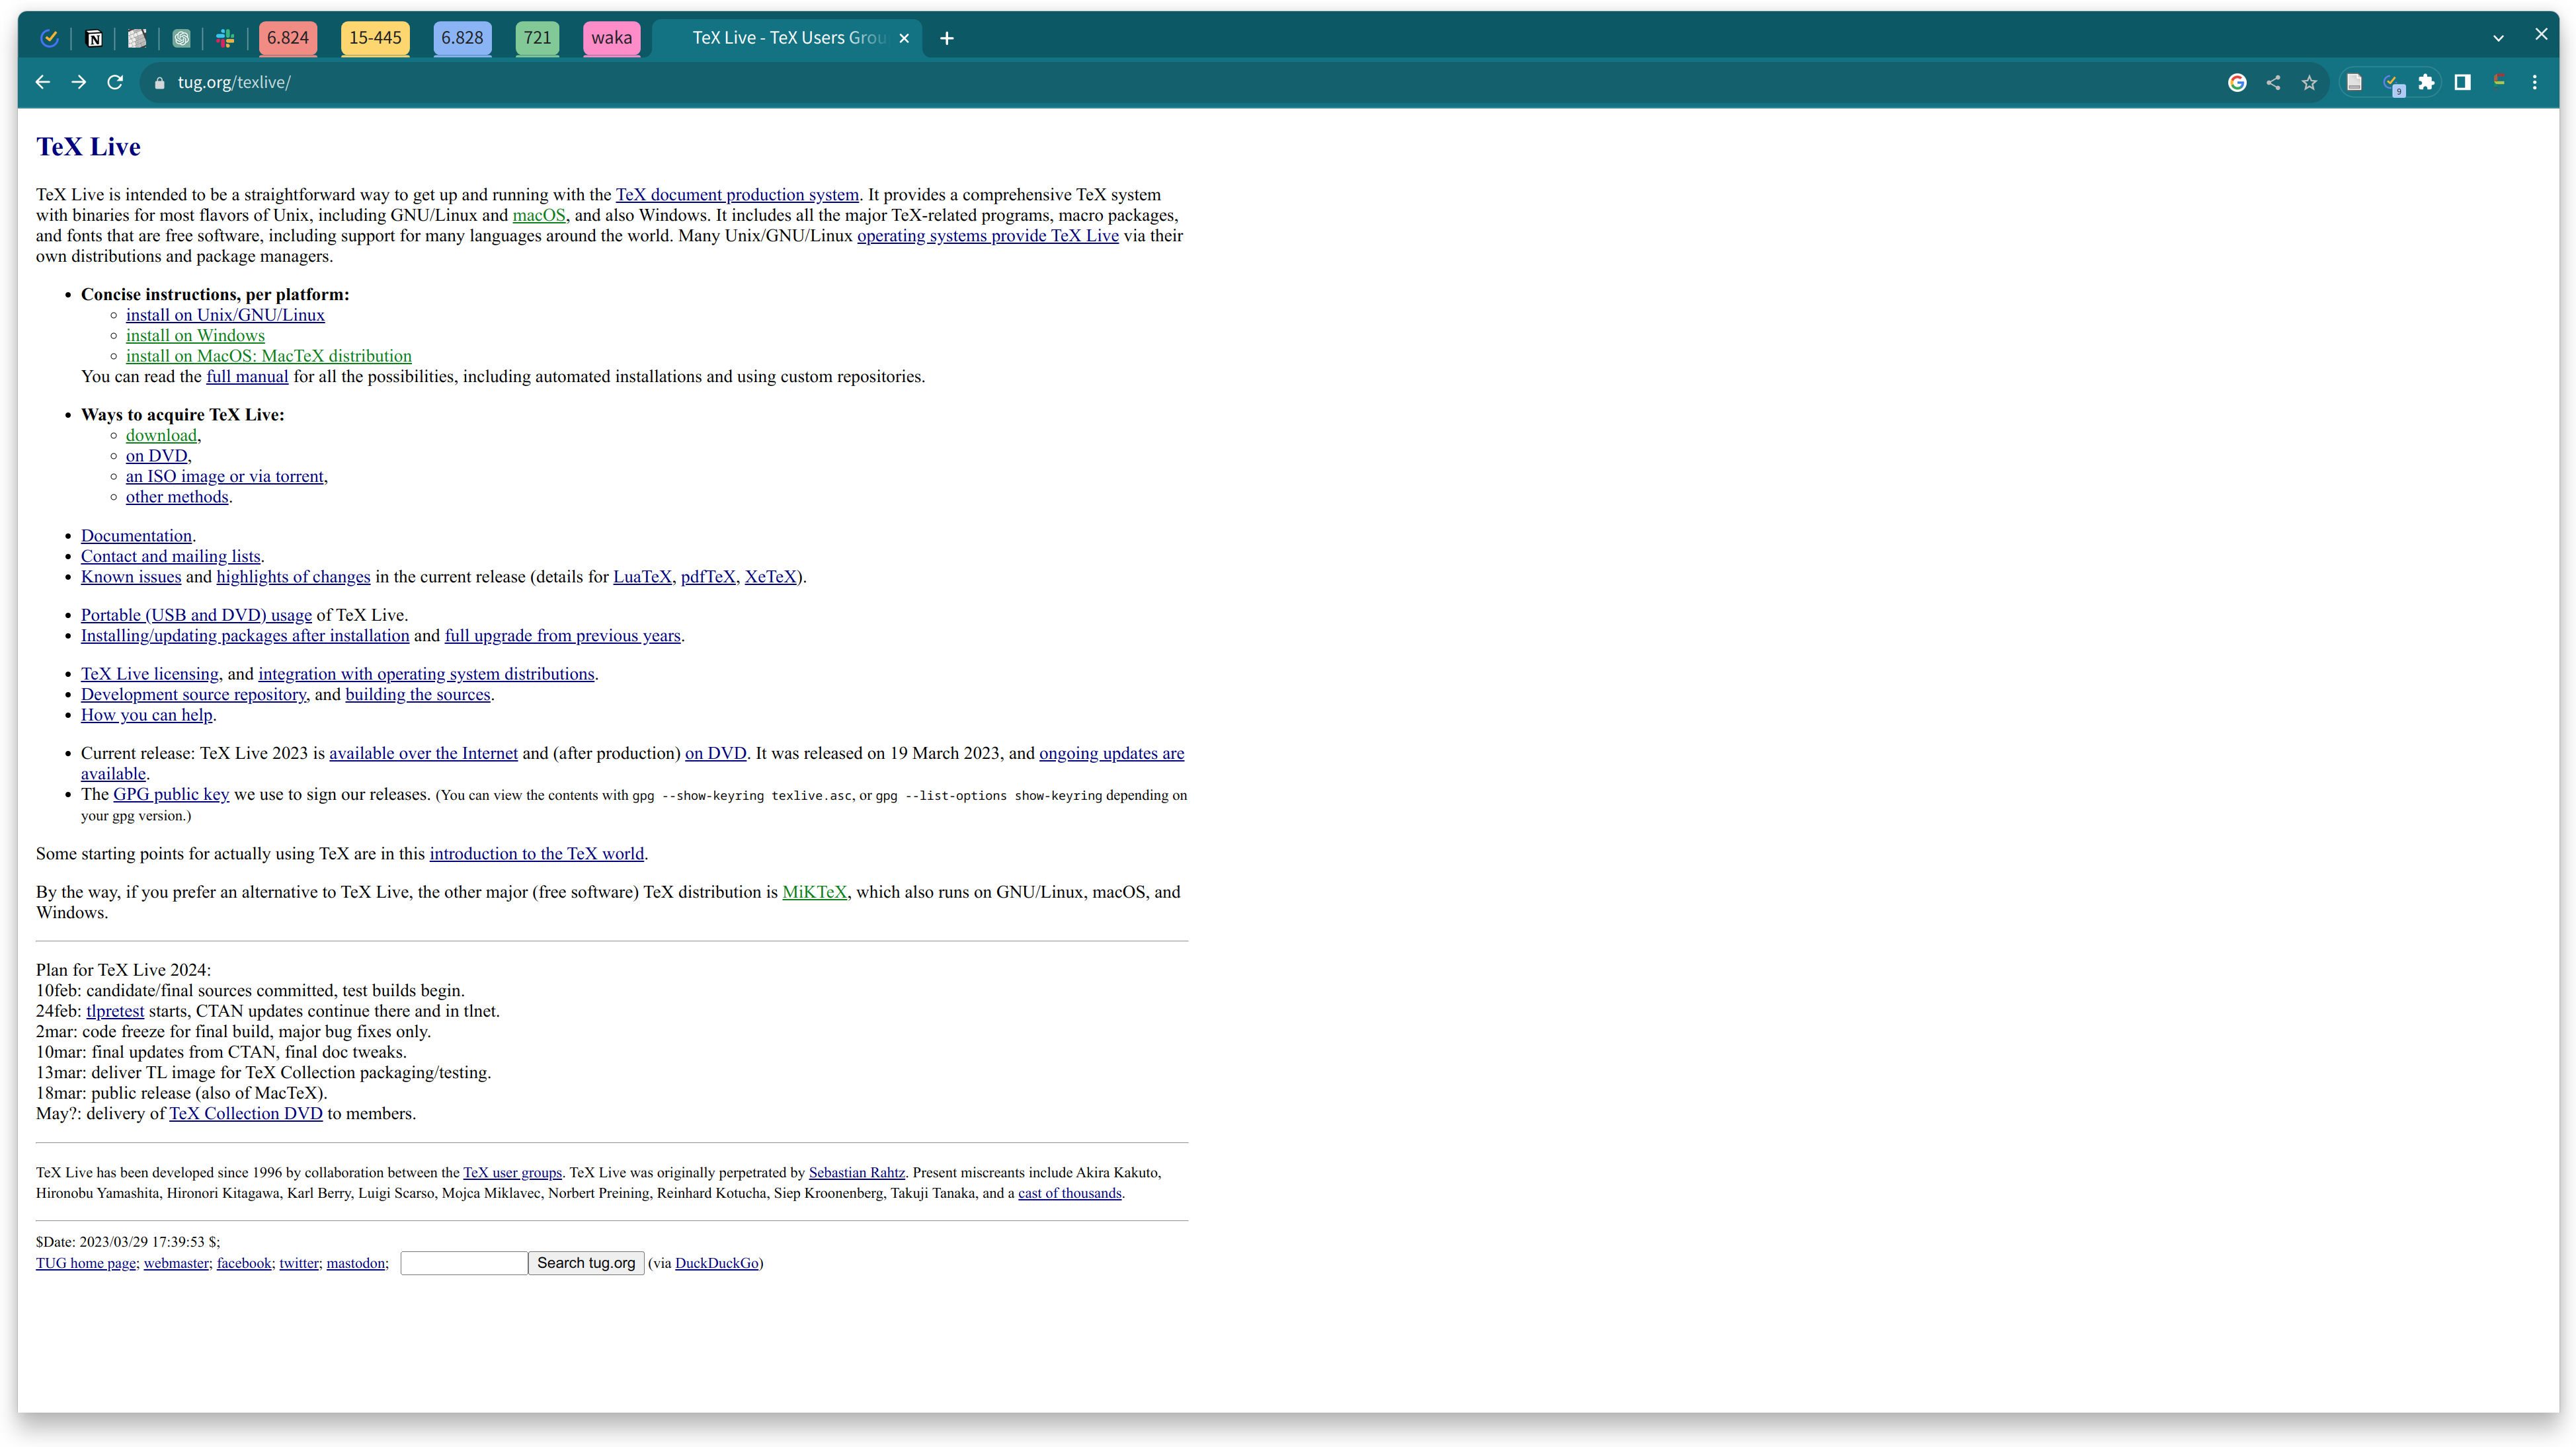
\includegraphics[width=0.85\textwidth]{imgs/local-texlive-download.png}
  \end{center}
  \caption{TeX Live 下载页面}
  \label{fig:local-texlive-download}
\end{figure}

\subsection{安装编辑器——TeXstudio}

访问 \url{https://www.texstudio.org/},下载并安装 TeXstudio。TeXstudio 是一个开源的、跨平台的、功能强大的 \LaTeX 编辑器。使用它,你可以更方便地进行 \LaTeX 的写作与编辑。

\begin{figure}[H]
  \begin{center}
    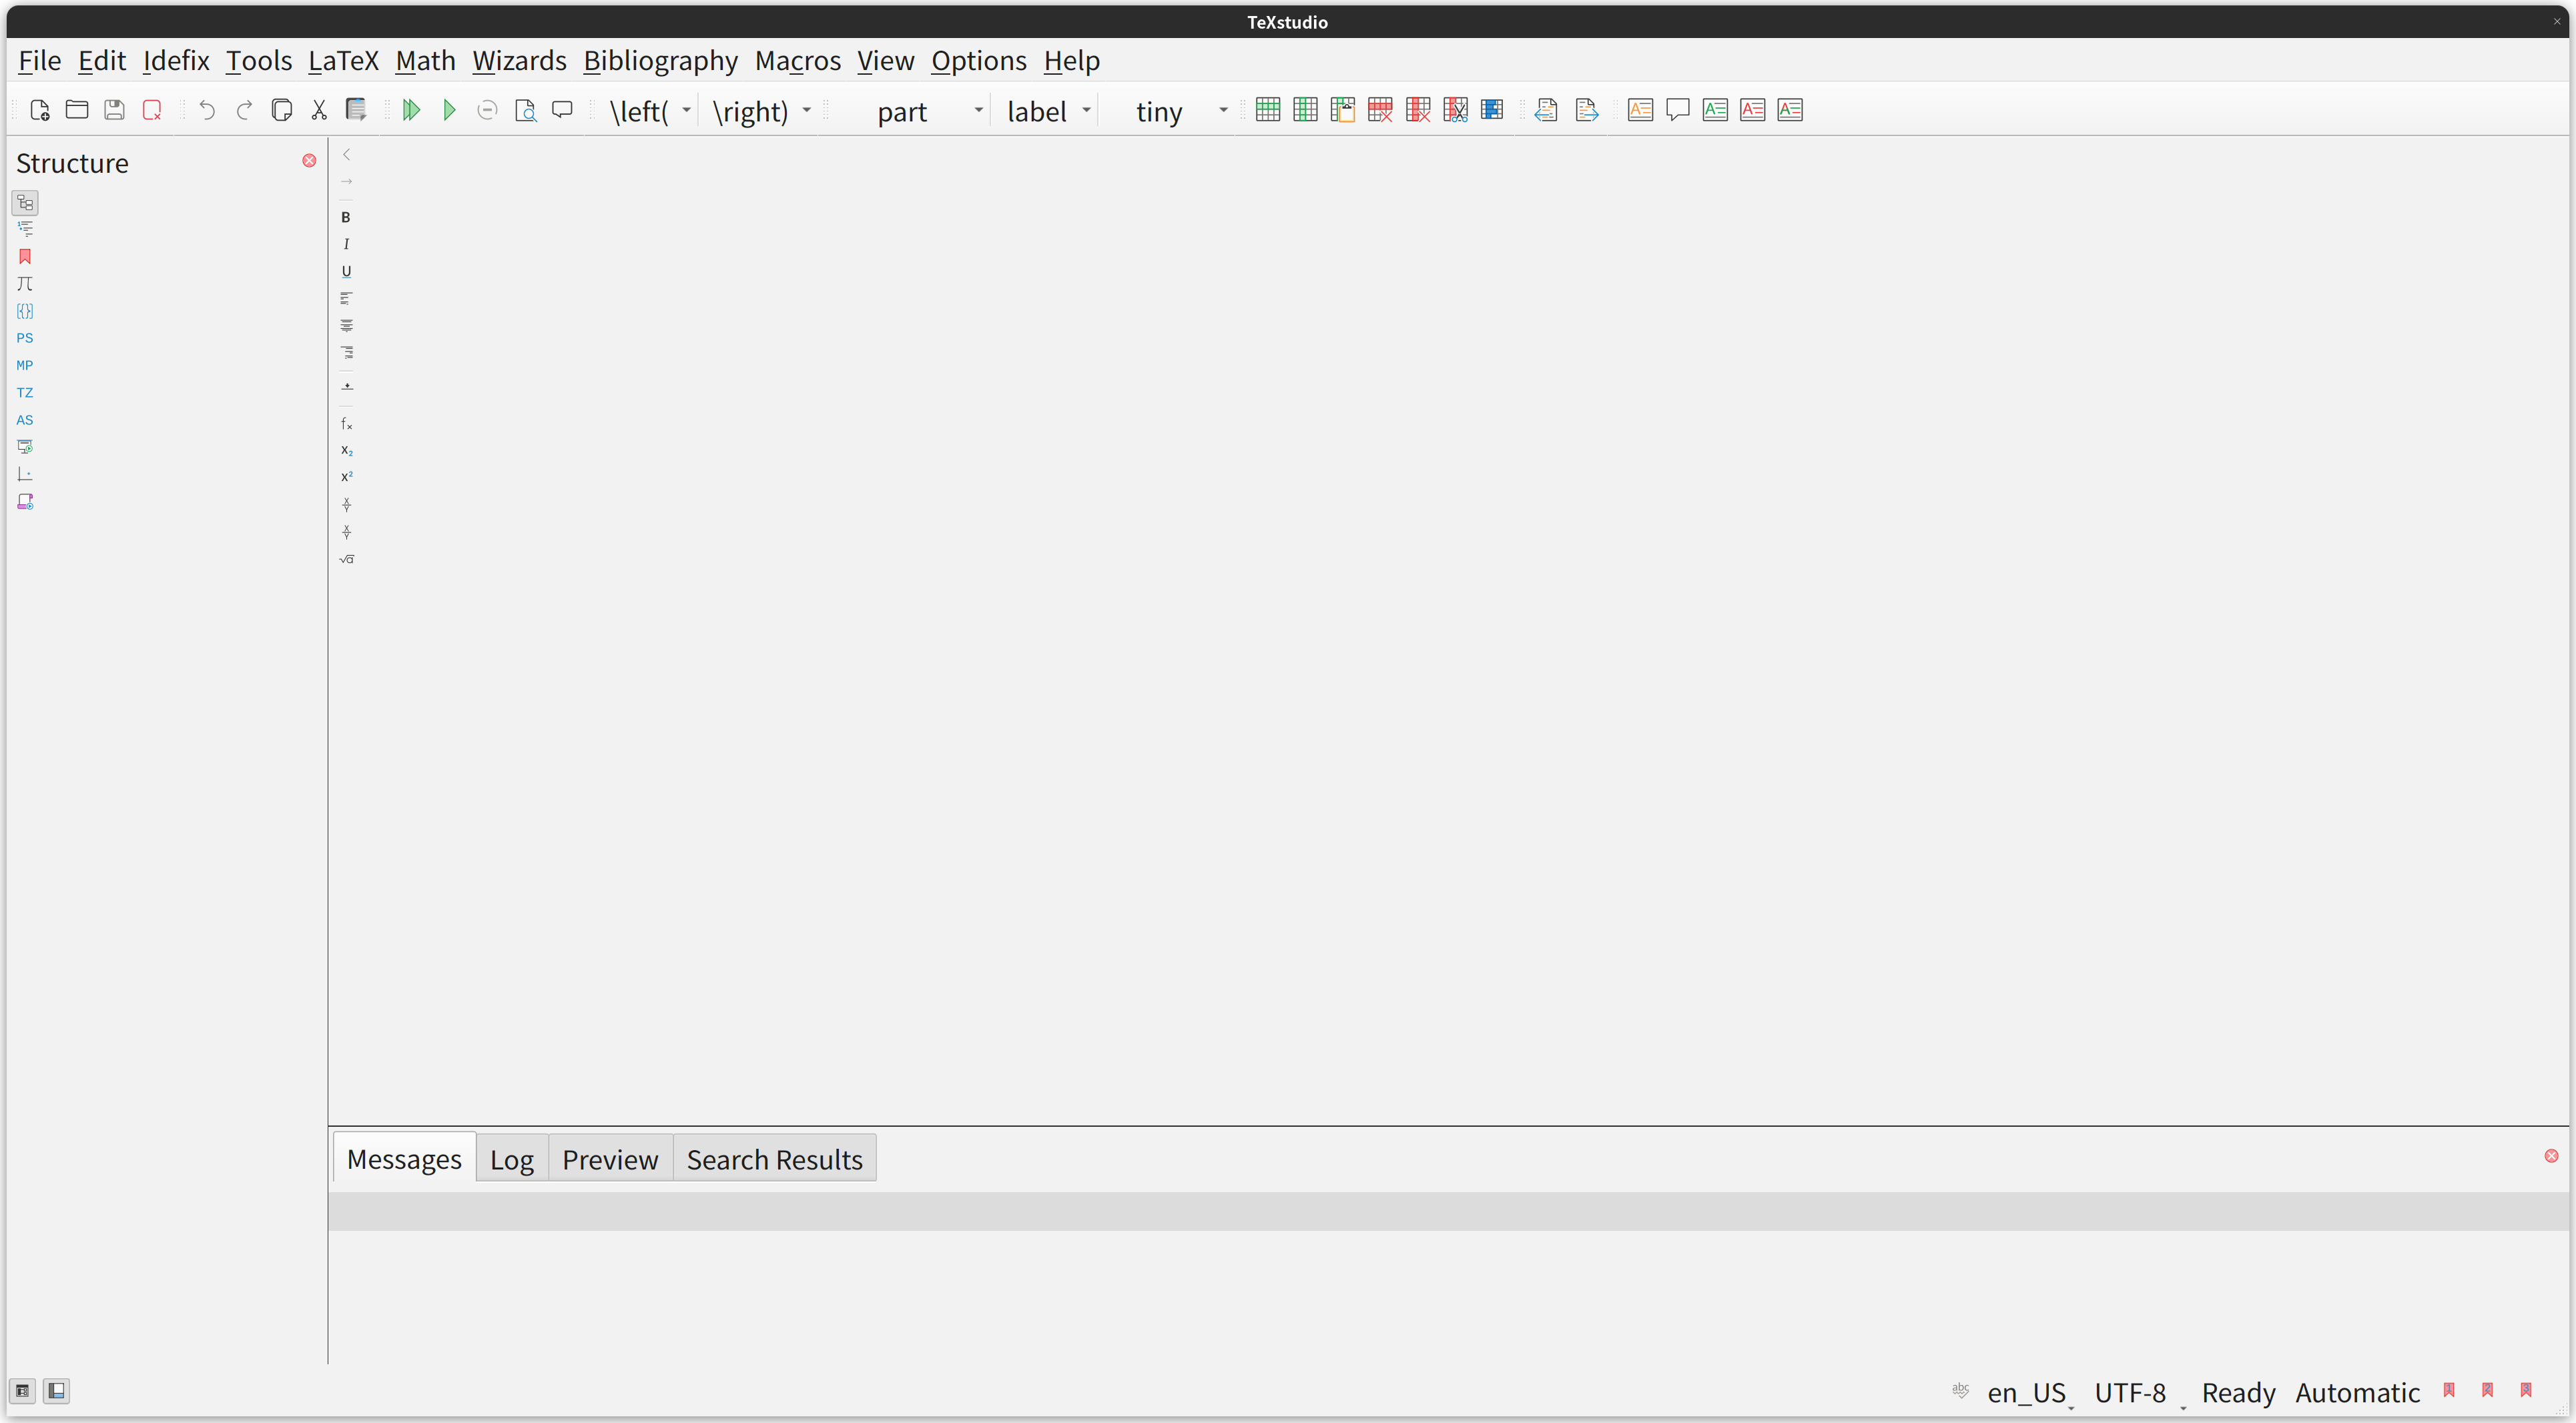
\includegraphics[width=0.85\textwidth]{imgs/texstudio-overview.png}
  \end{center}
  \caption{TeXstudio 界面}
  \label{fig:texstudio-overview}
\end{figure}

\subsection{下载模板}

\textit{如果你选择使用目前版本的模板,可以跳过该步骤。}

访问 \url{https://bithesis.bitnp.net},点击右上角的“模板下载”,跳转到 \BIThesis 项目的 GitHub Releases 页面(也即 \url{https://github.com/BITNP/BIThesis/releases/latest})。选择\isGraduateTF{``graduate-thesis.zip''}{``undergraduate-thesis.zip''}的模板压缩包并下载。

\isGraduateTF{}{
  \textit{若为全英文专业,请选择``undergraduate-thesis-en.zip''。}
}

\begin{figure}[H]
  \begin{center}
    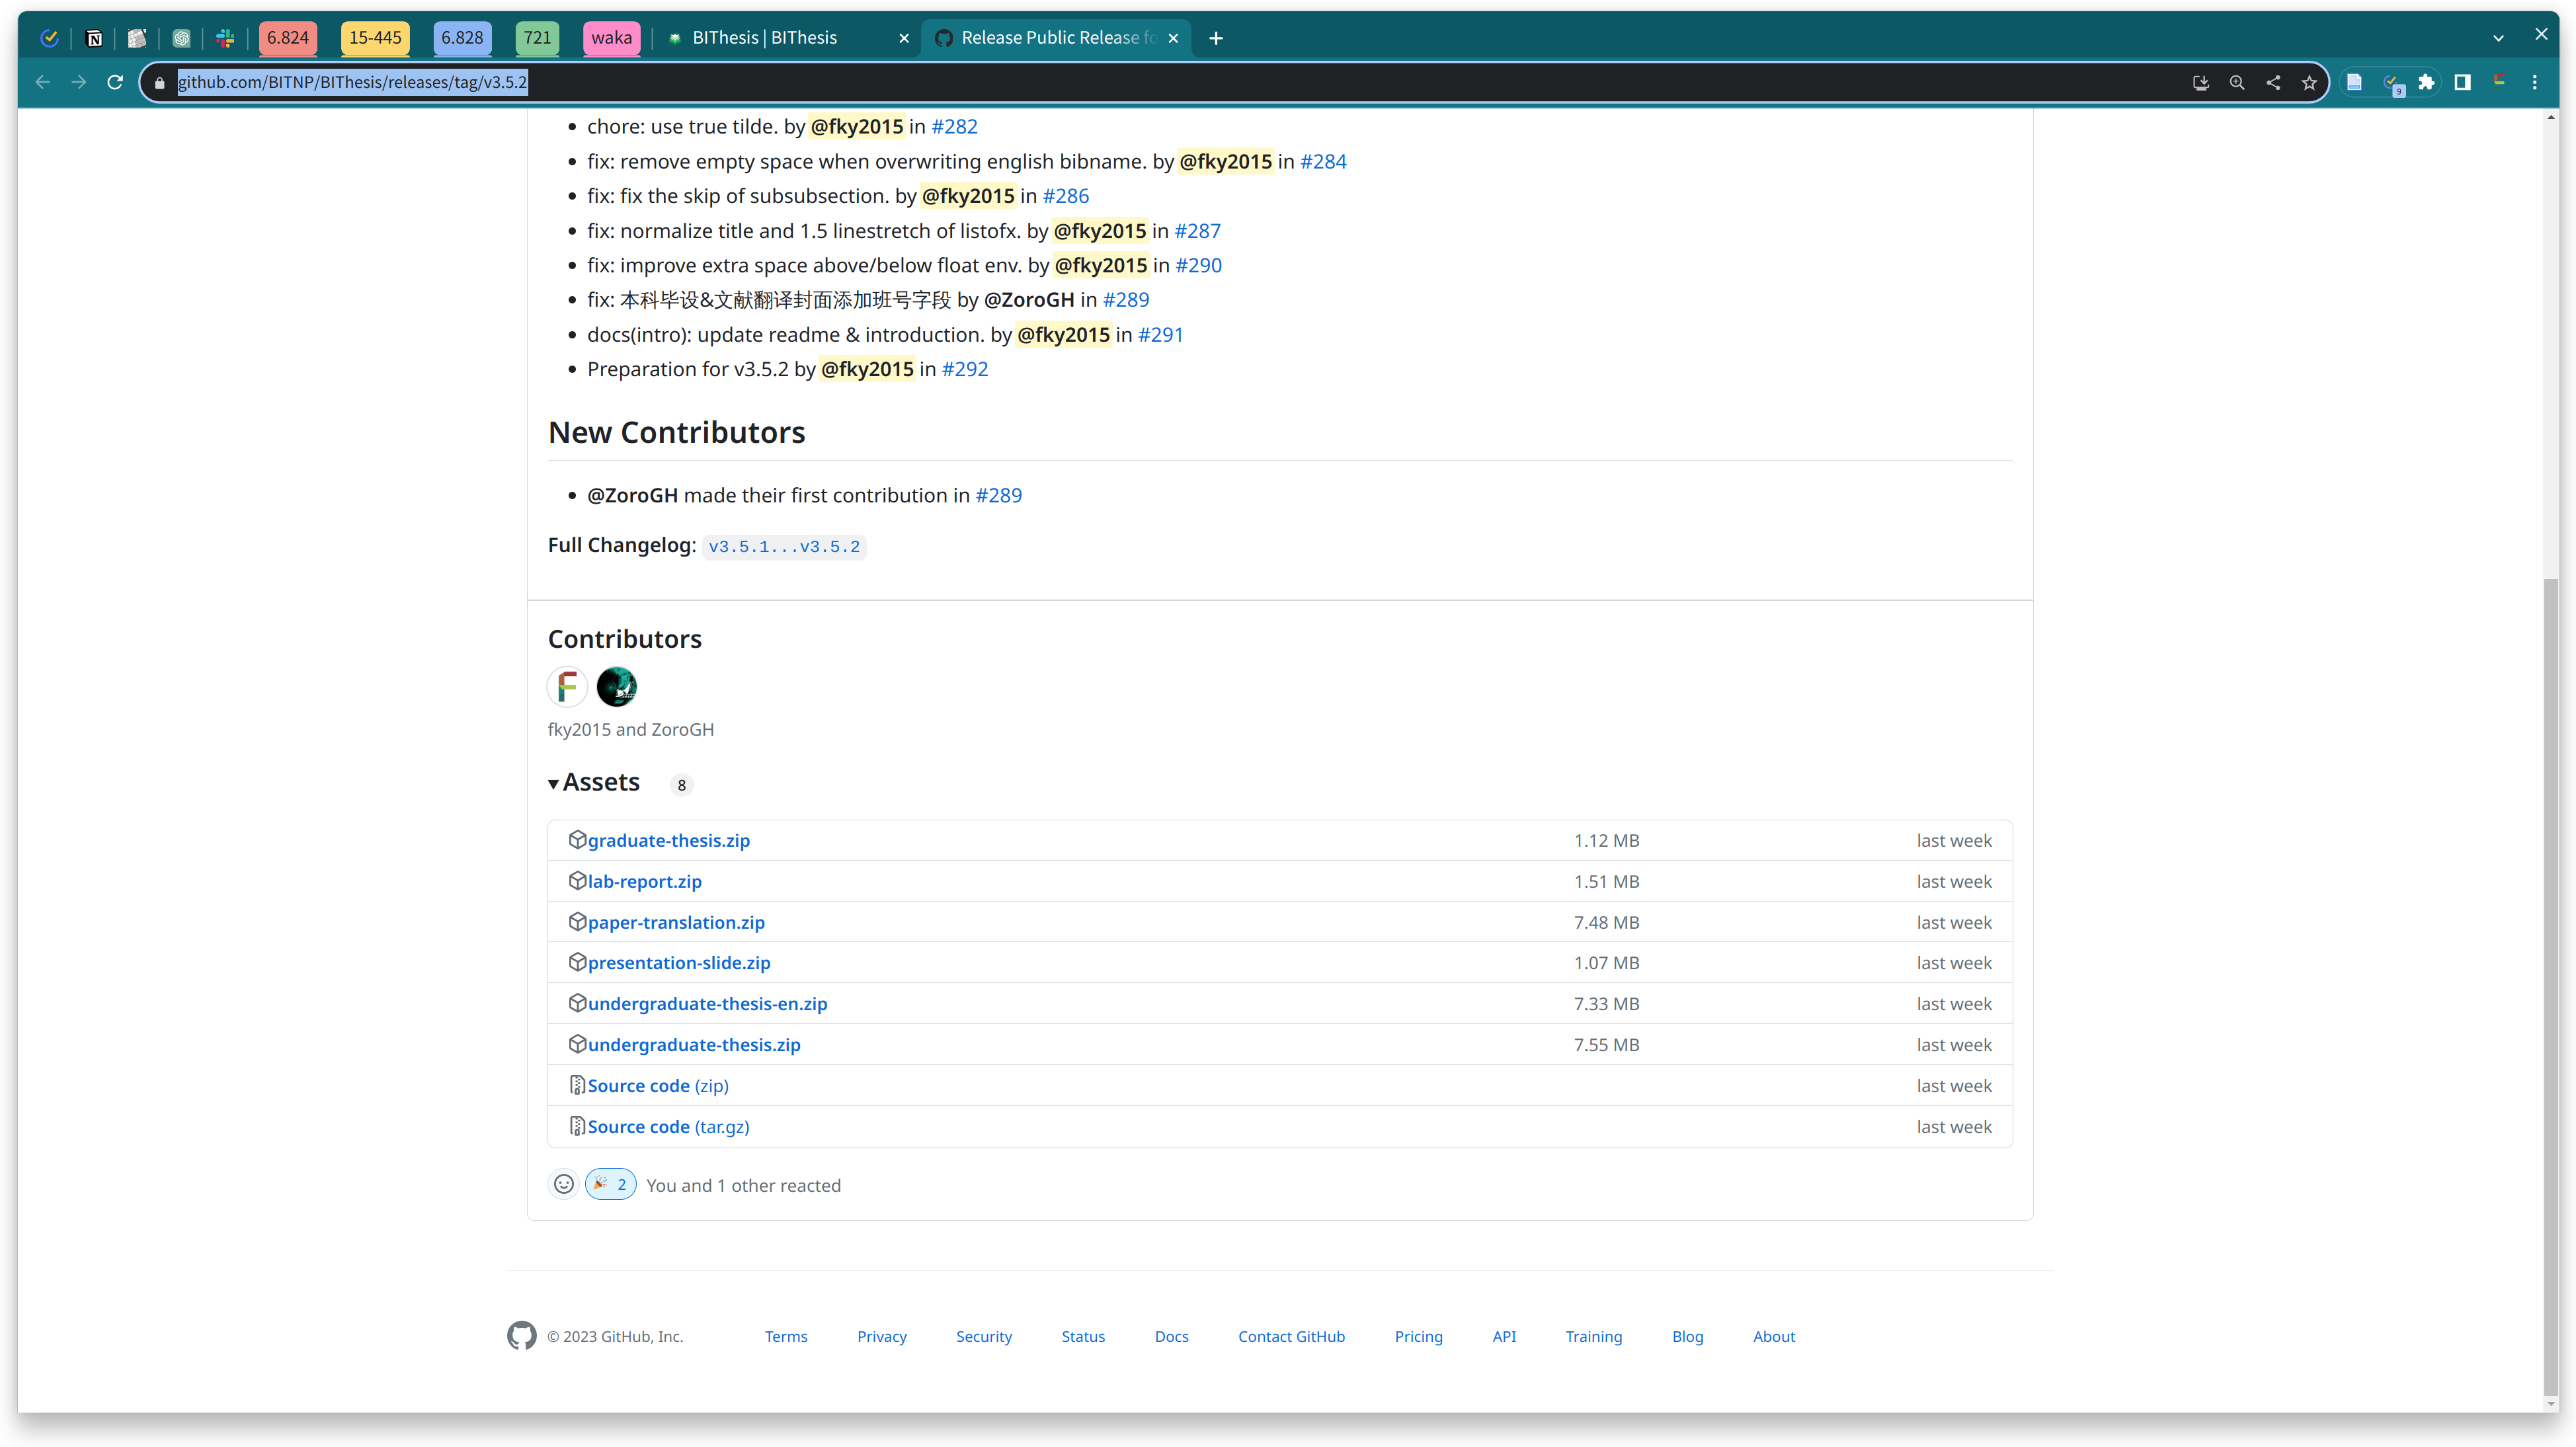
\includegraphics[width=0.85\textwidth]{imgs/github-releases.png}
  \end{center}
  \caption{模板下载页面}
  \label{fig:local-template-download}
\end{figure}

\subsection{编译生成 PDF}

解压模板压缩包,打开 TeXstudio,点击 ``File > Open'' 按钮,选择 ``main.tex'' 文件,即可打开模板。

接着,点击 ``Build \& View'' 按钮(两个叠加的绿色三角),即可编译生成 PDF。

\begin{figure}[H]
  \begin{center}
    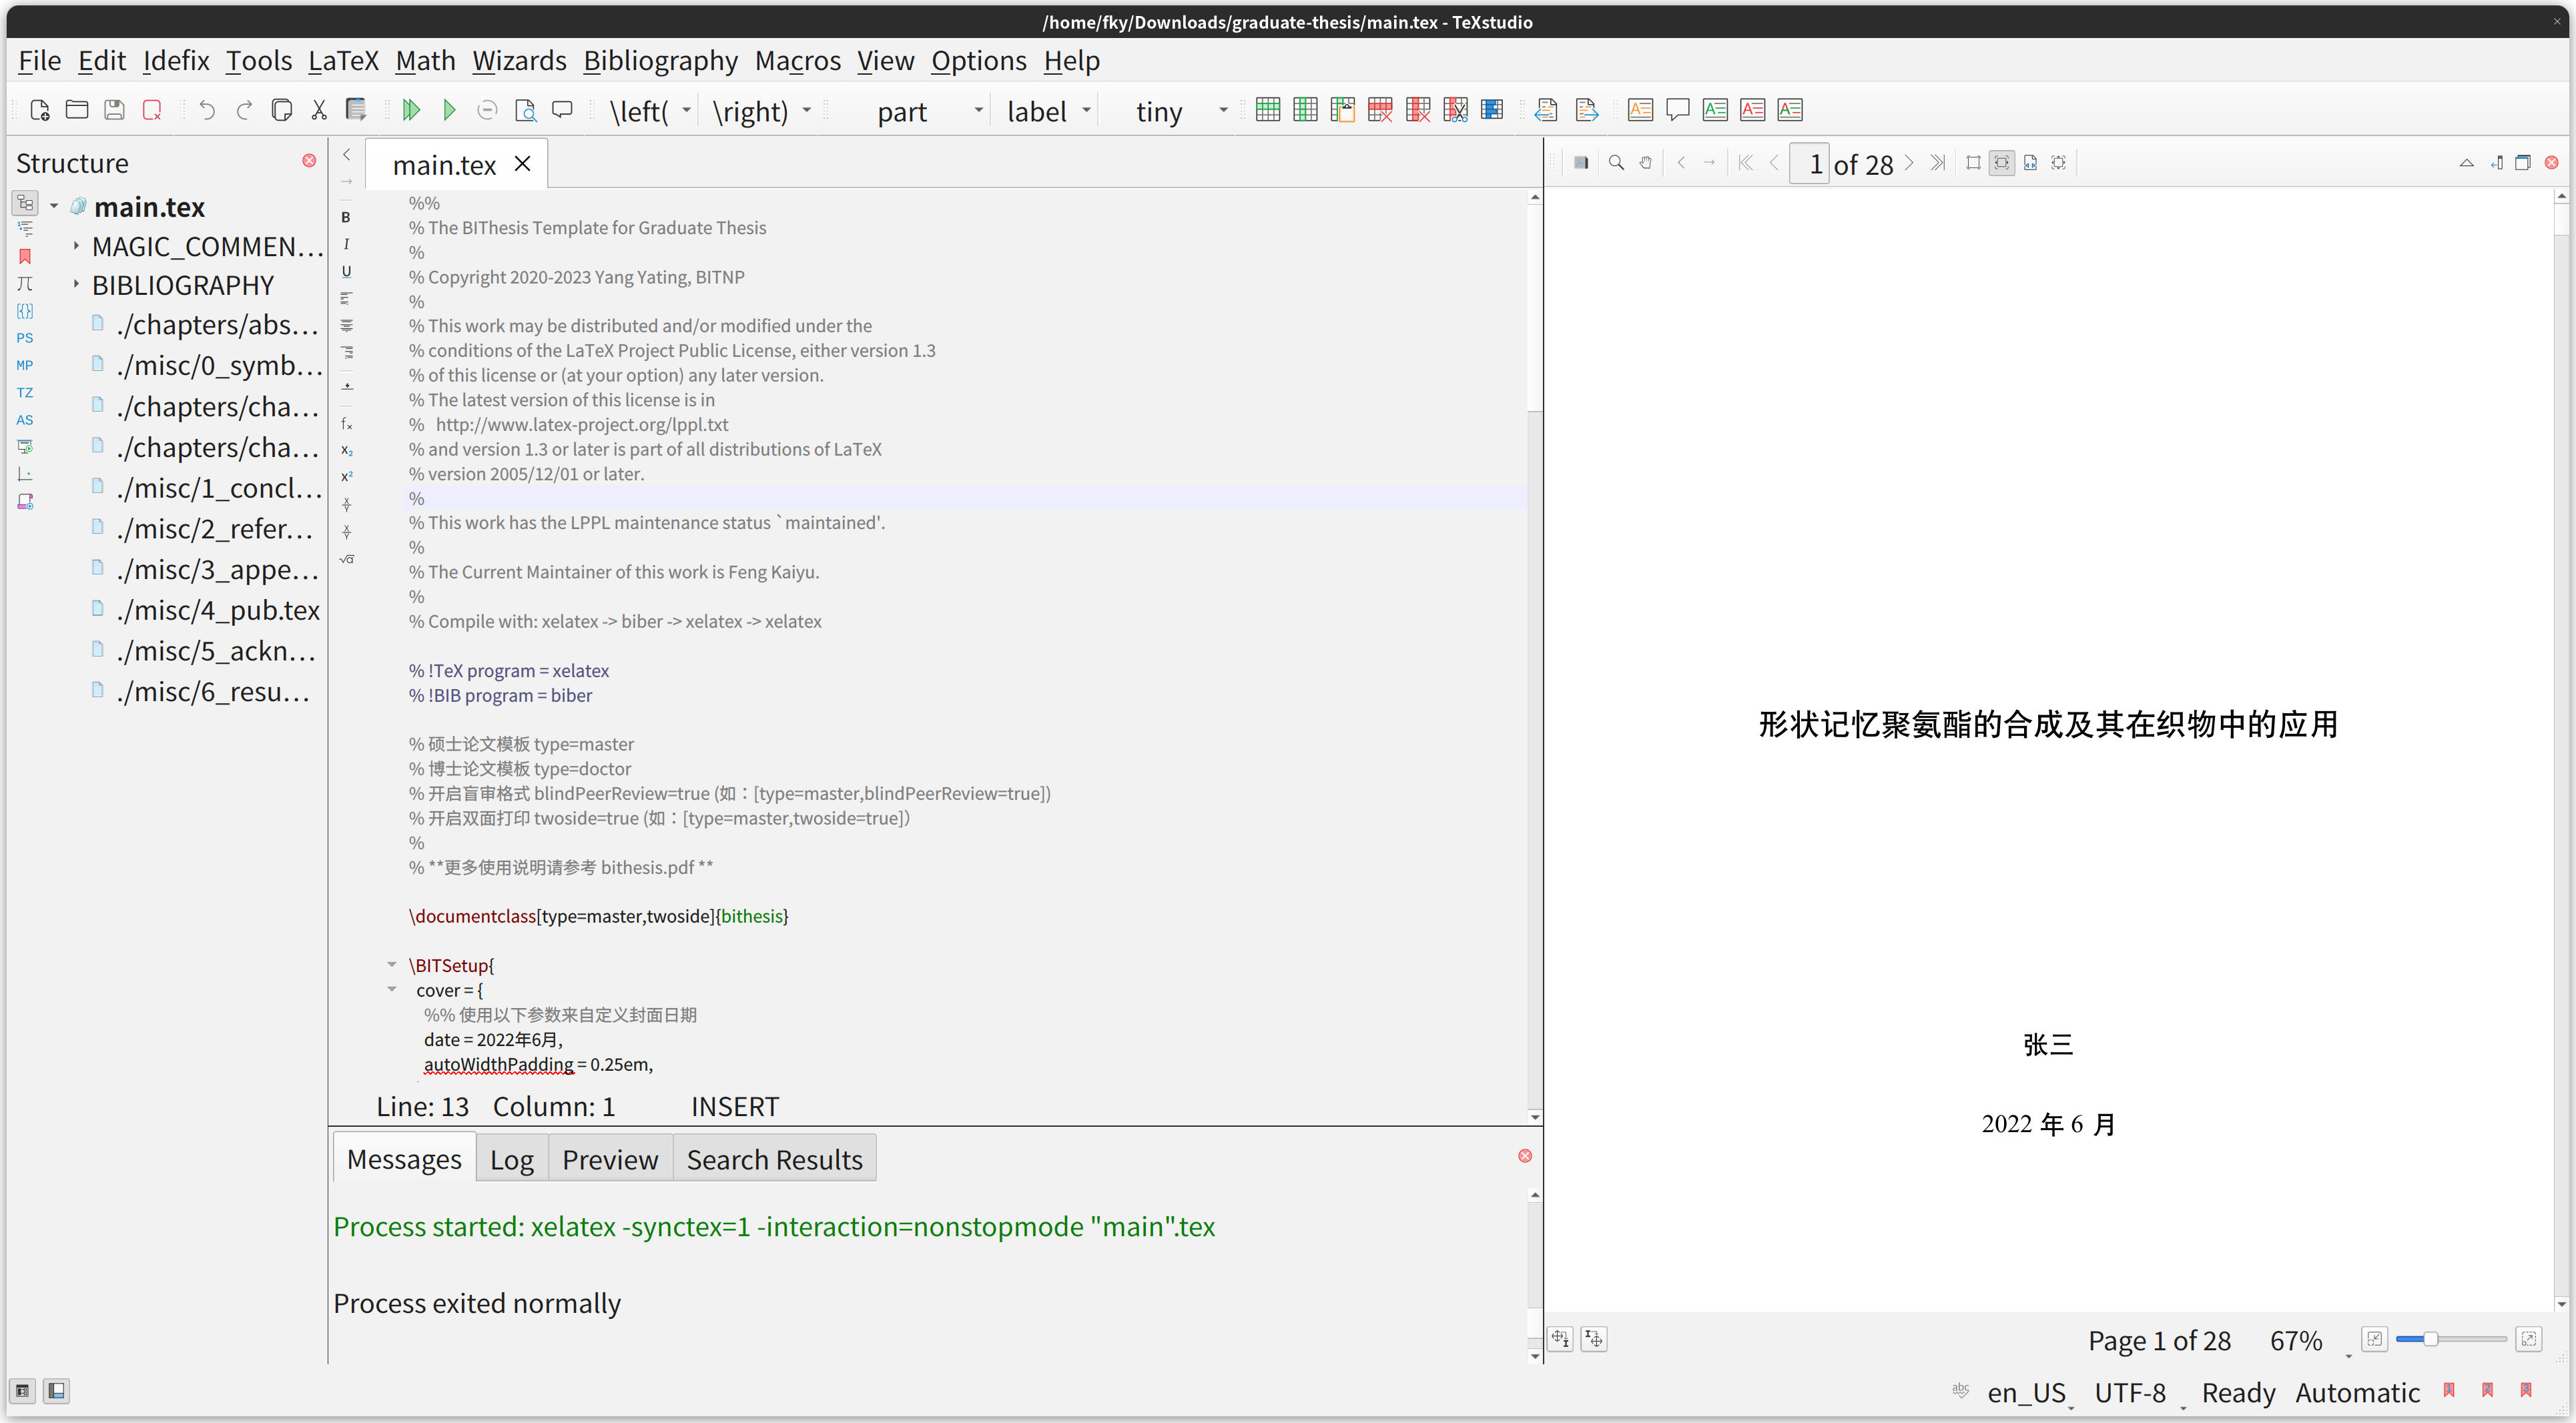
\includegraphics[width=0.85\textwidth]{imgs/texstudio-compile-and-view.png}
  \end{center}
  \caption{TeXstudio 编译生成 PDF}
  \label{fig:texstudio-compile-and-view}
\end{figure}

\section{方法二:在 Overleaf(浏览器)上编译生成 PDF}
\label{sec:overleaf-compile}

\BIThesis 项目已经在 Overleaf 上分享了多个模板,它们
会与最新版本保持同步\footnote{需要注意,你复制的模板不会自动更新。}。
因此,你可以直接在 Overleaf 上复制并使用这些模板。

\subsection{注册 Overleaf 账号}

访问 \url{https://overleaf.com}(如\autoref{fig:overleaf-register}所示),点击右上角的 ``Register'' 按钮,注册账号并登录。

\begin{figure}[H]
  \begin{center}
    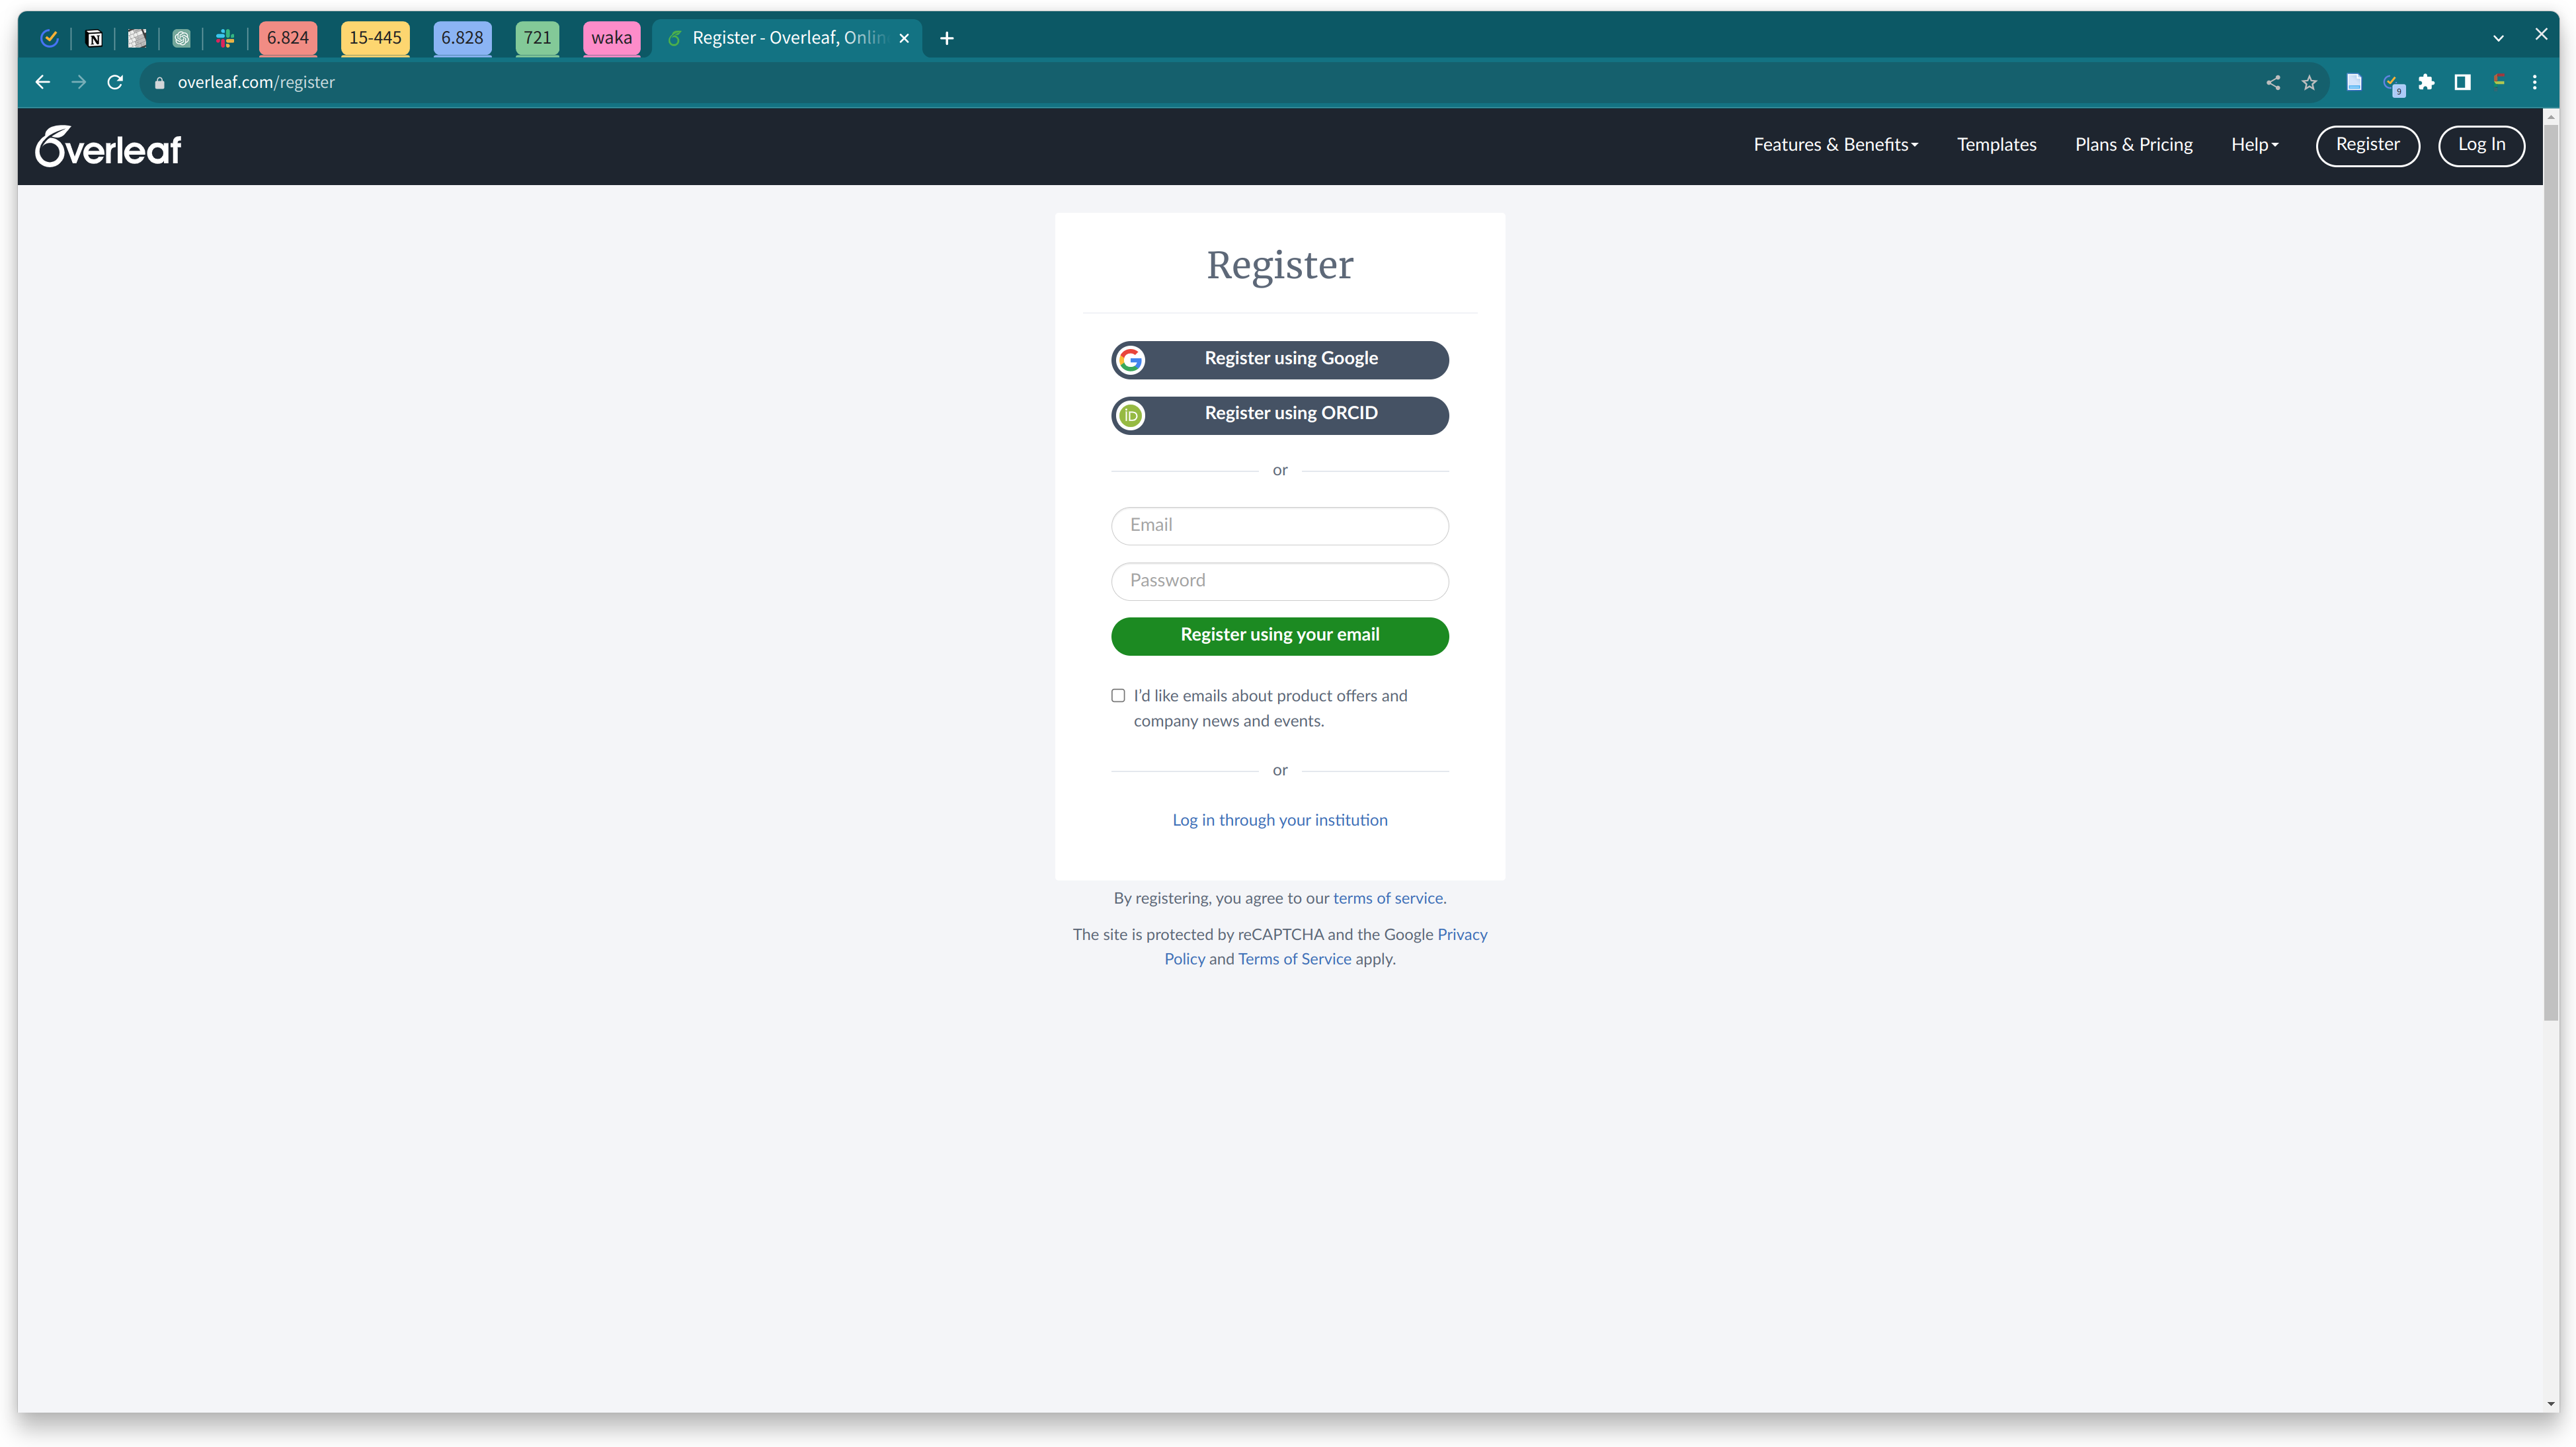
\includegraphics[width=0.85\textwidth]{imgs/overleaf-register.png}
  \end{center}
  \caption{Overleaf 注册页面}
  \label{fig:overleaf-register}
\end{figure}


\subsection{访问 \BIThesis 的 Overleaf 模板}

访问 \url{https://bithesis.bitnp.net},点击右上角的 ``Overleaf'' ,即可跳转到模板页面。

选择\isGraduateTF{“研究生学位论文模板”}{“本科生毕业设计论文模板”}模板,点击 ``Open in Overleaf'' 按钮,即可跳转到 Overleaf 上分享的项目中。

\isGraduateTF{}{
  \textit{若为全英文专业,请选择“本科生毕业设计论文模板(全英文专业)”。}
}

\begin{figure}[H]
  \begin{center}
    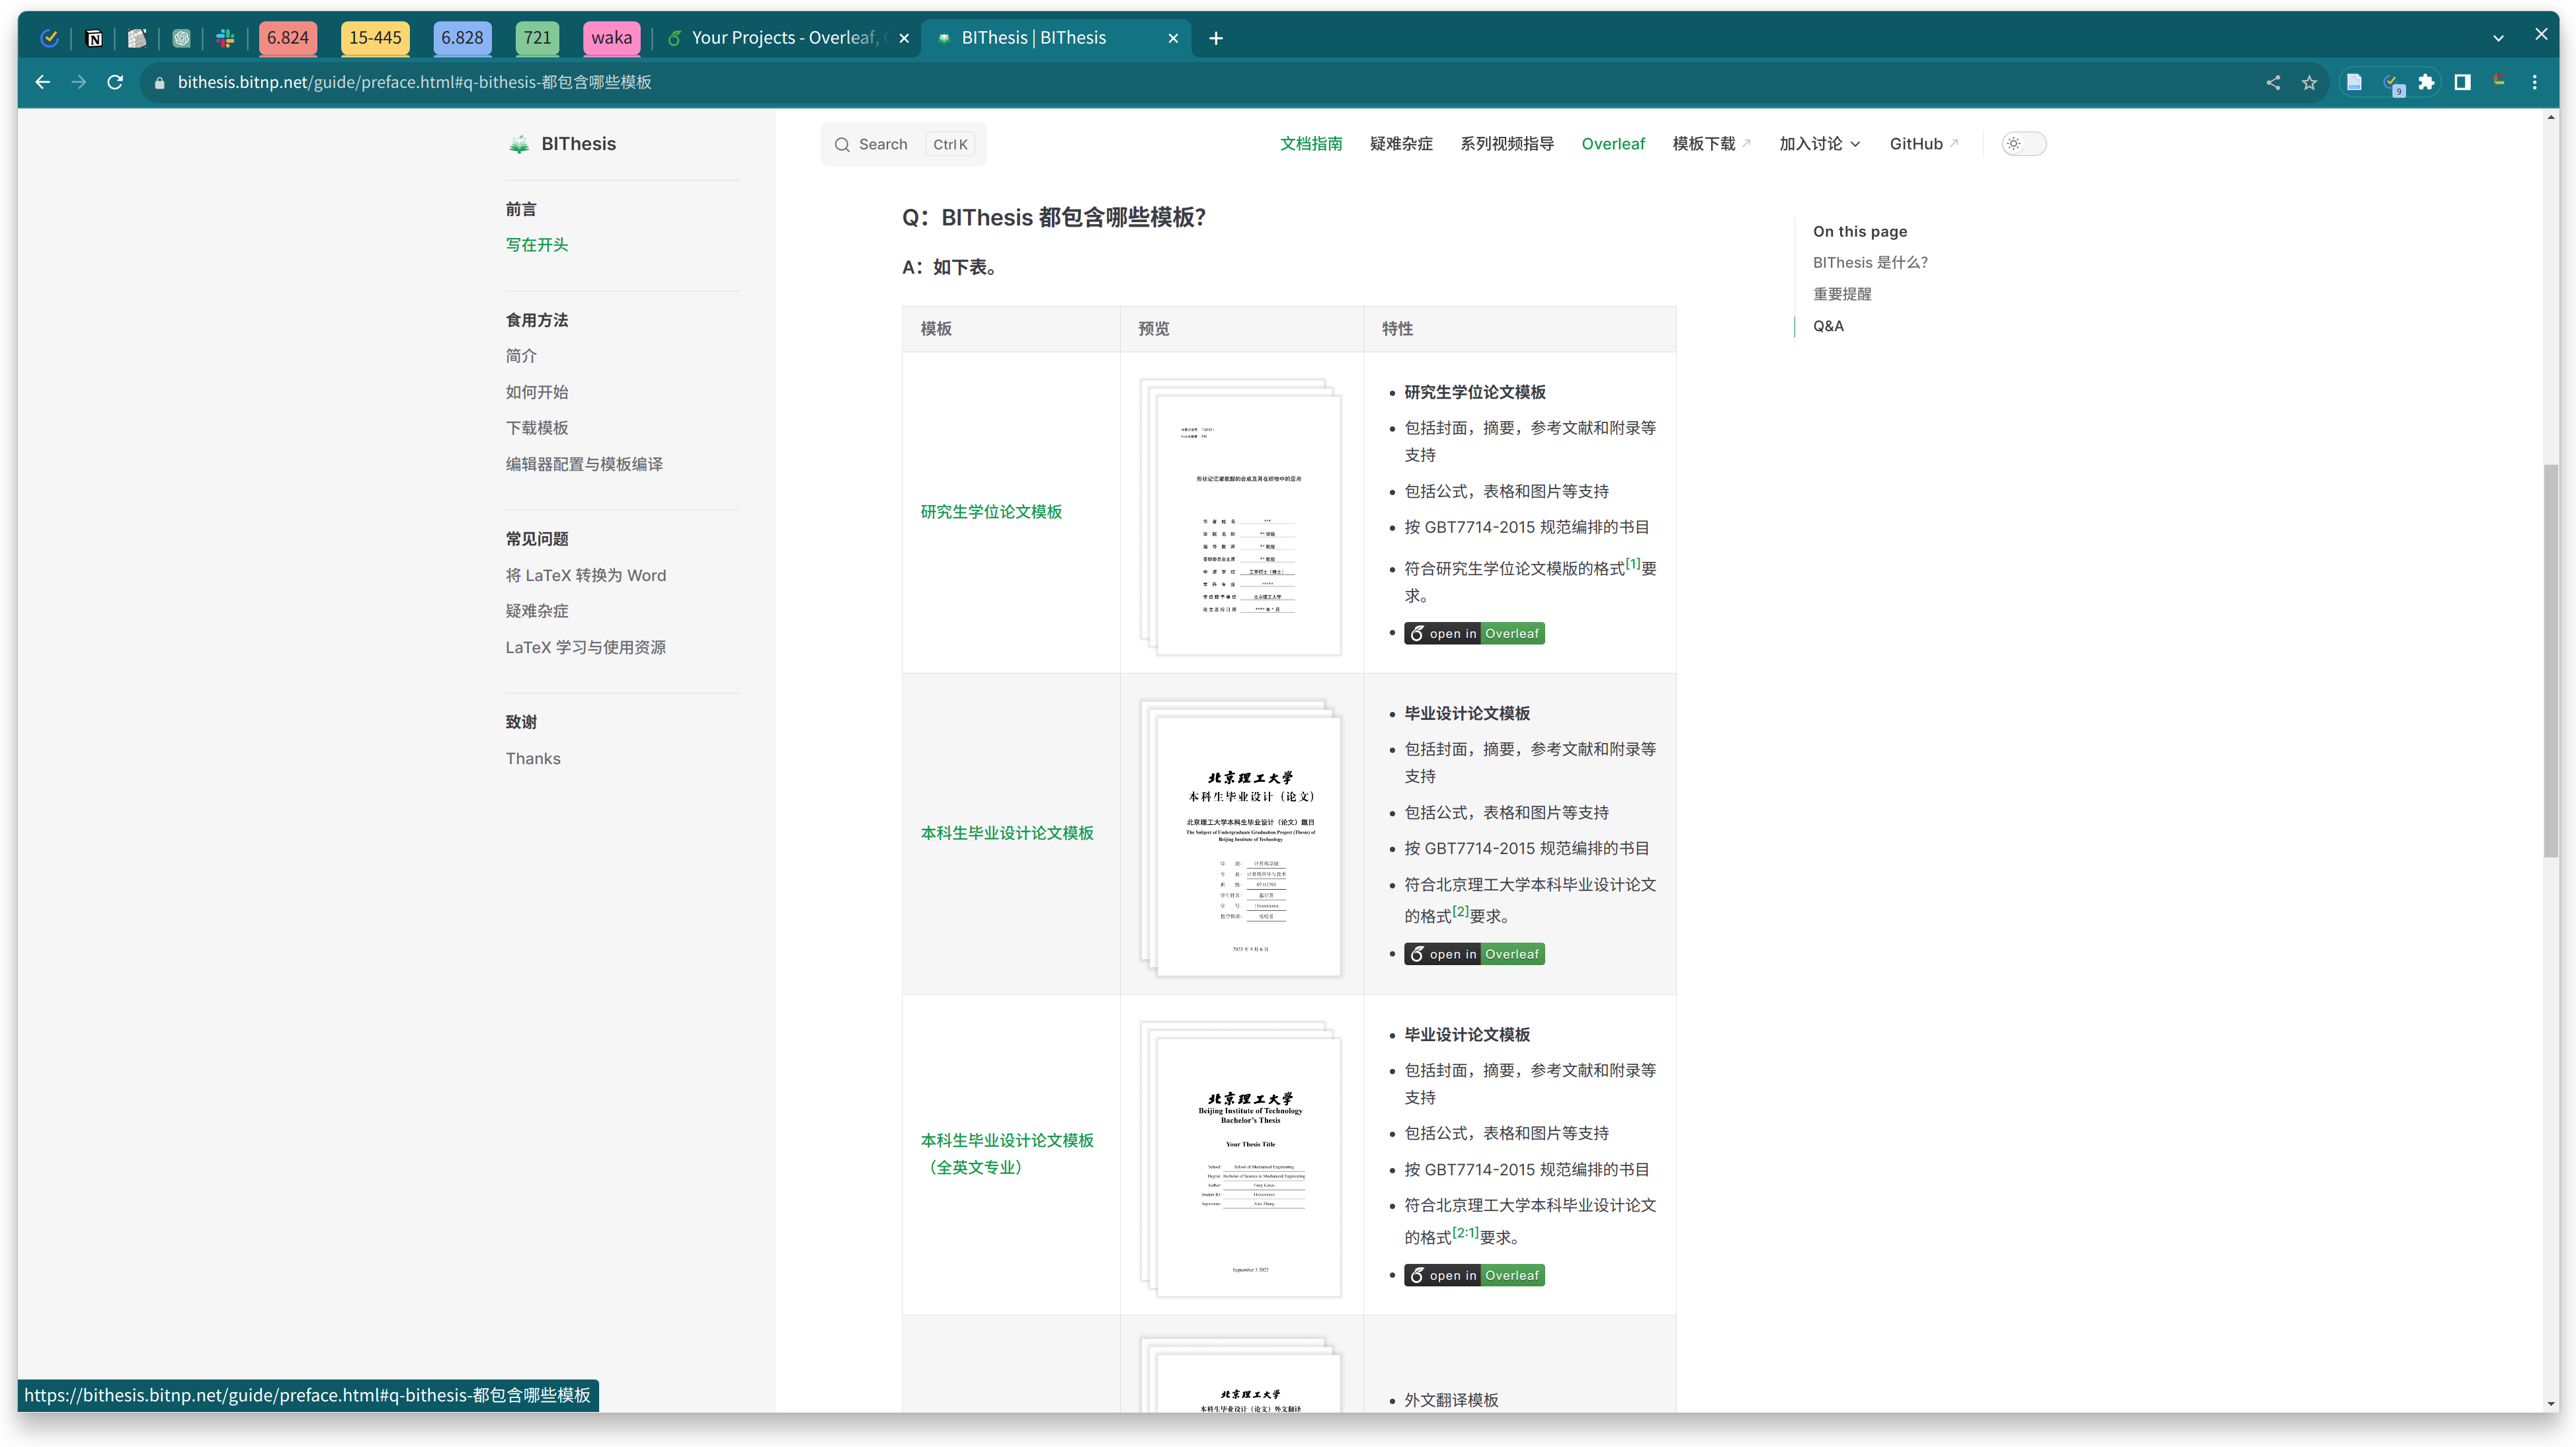
\includegraphics[width=0.85\textwidth]{imgs/overleaf-choose-template.png}
  \end{center}
  \caption{在 BIThesis-wiki 中,选择合适的模板并跳转}
  \label{fig:overleaf-template}
\end{figure}

\subsection{编译生成 PDF}

点击 ``Recompile'' 按钮,即可编译生成 PDF。

\begin{figure}[H]
  \begin{center}
    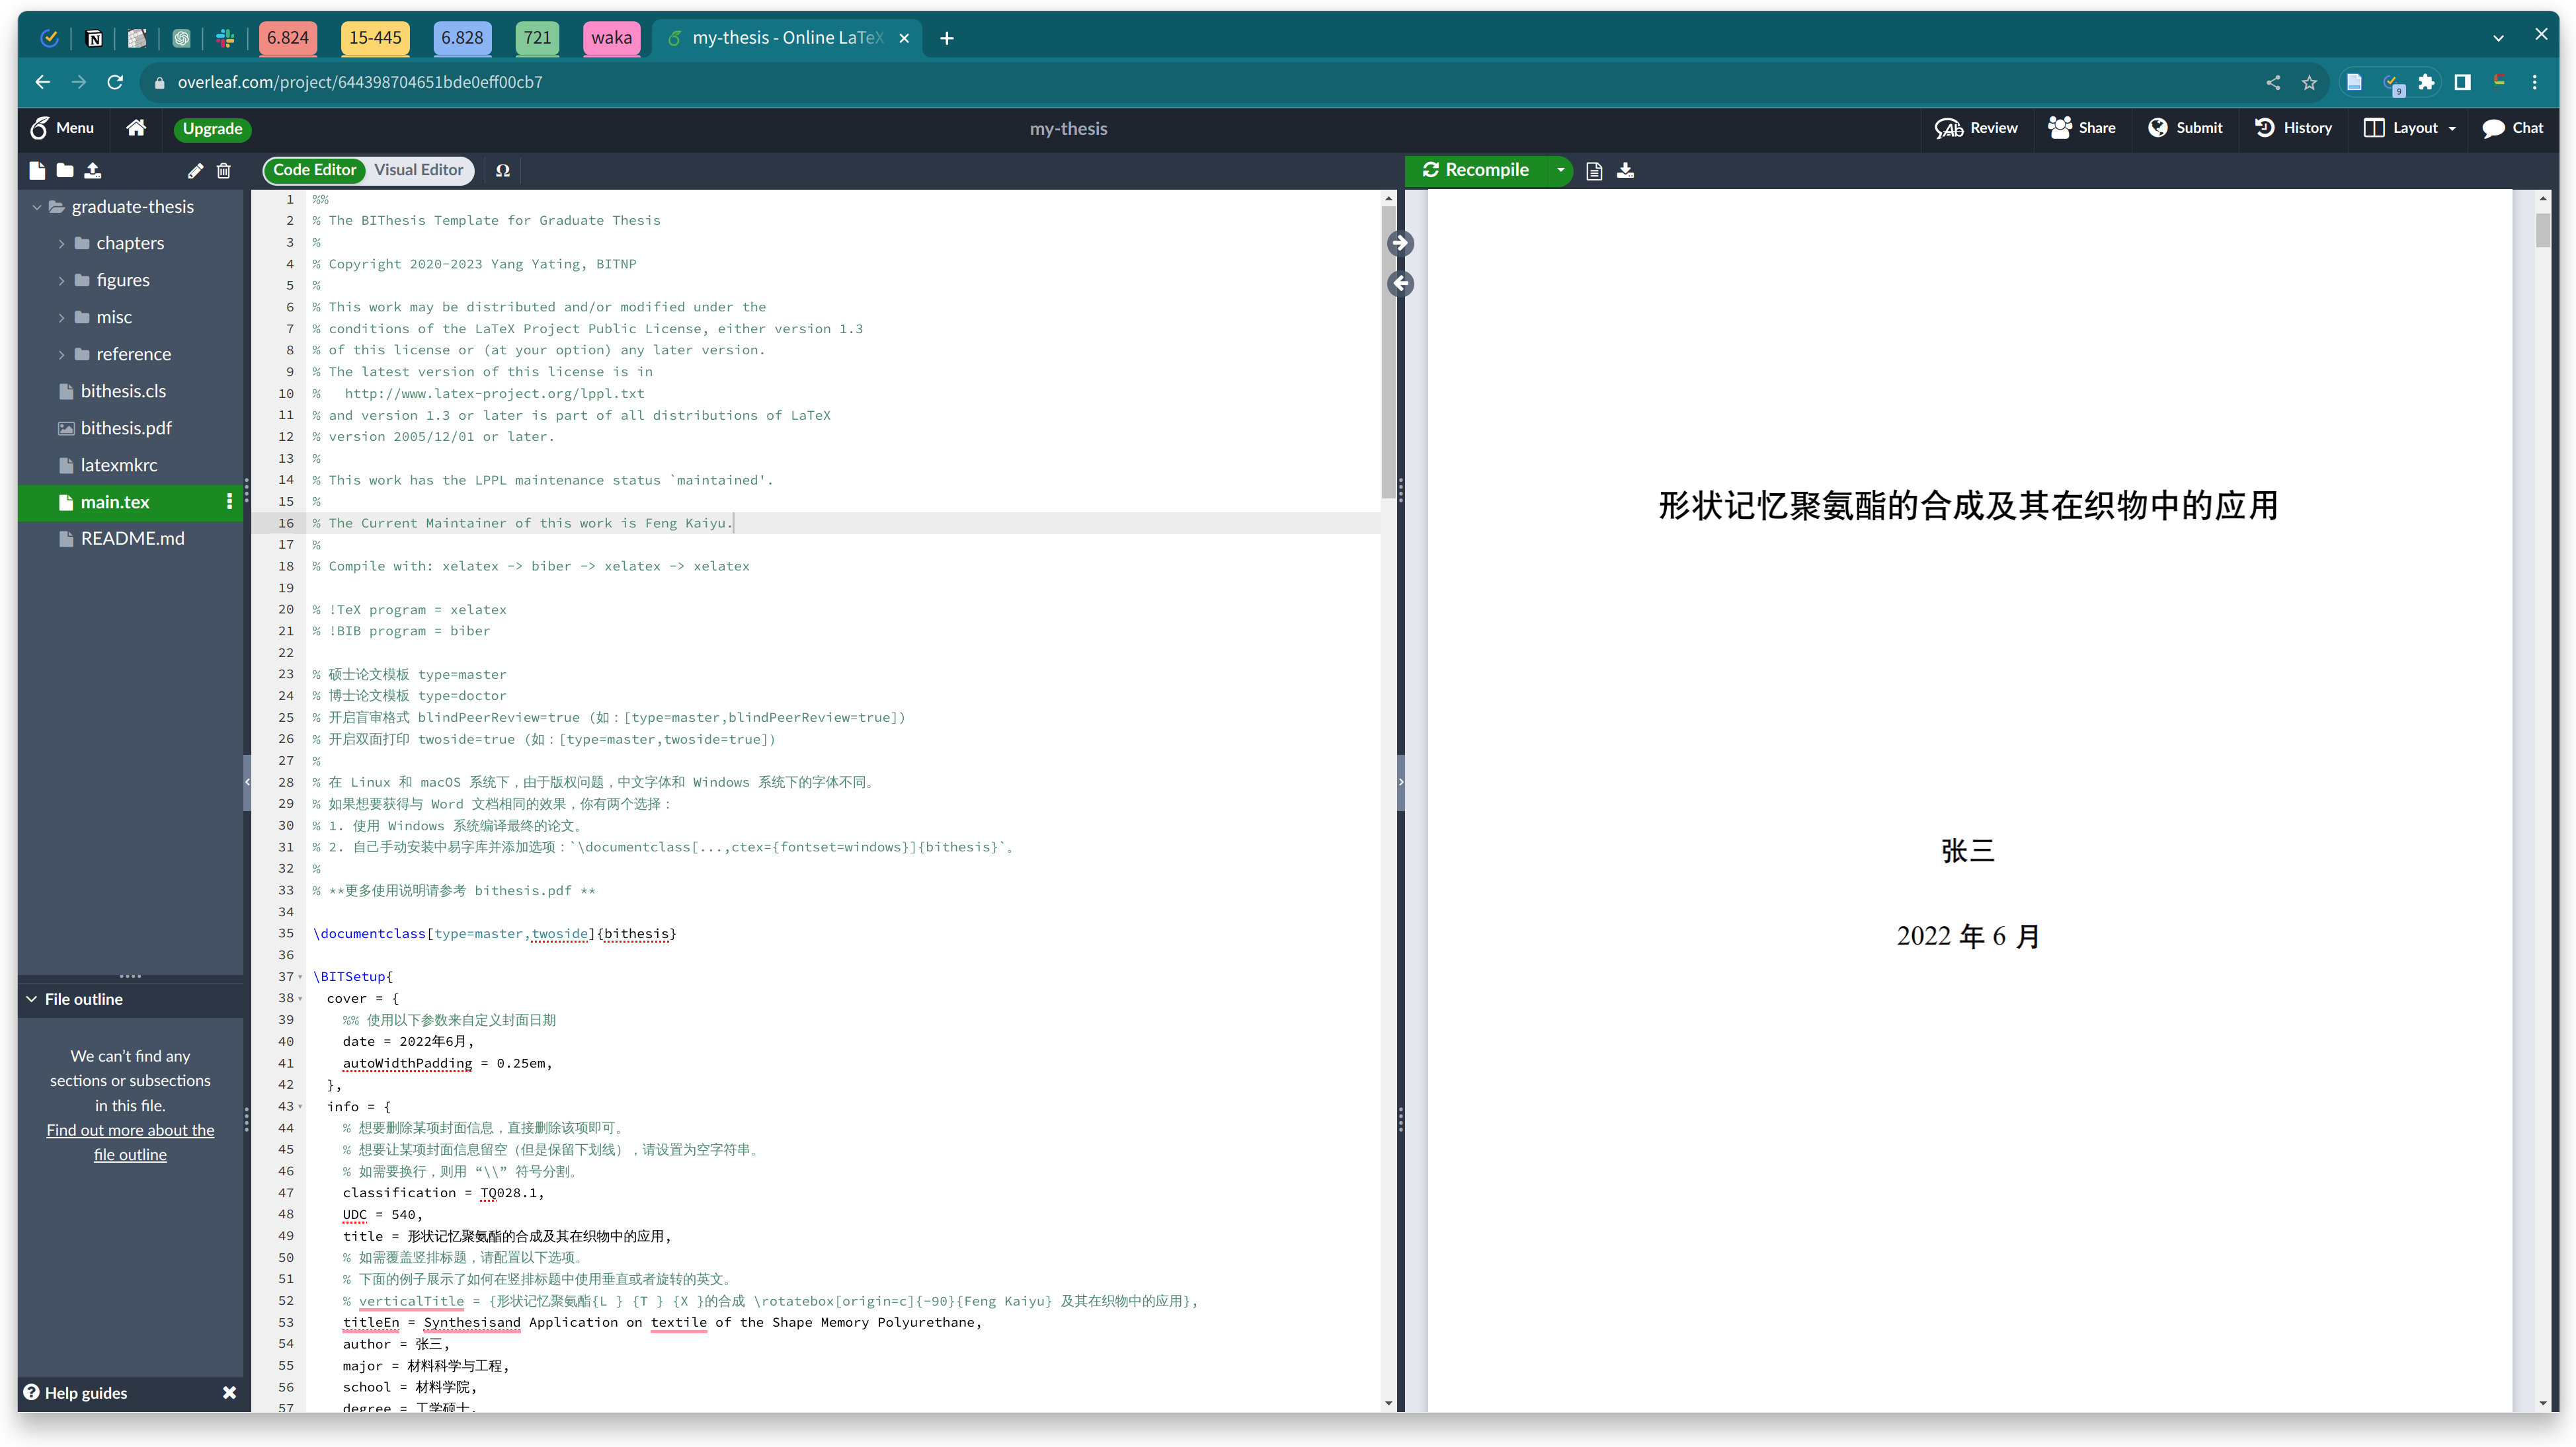
\includegraphics[width=0.85\textwidth]{imgs/overleaf-compile.png}
  \end{center}
  \caption{编译生成 PDF}
  \label{fig:overleaf-recompile}
\end{figure}

